\documentclass[../main.tex]{subfiles}
\graphicspath{{\subfix{../figures/}}}

\begin{document}
The first step towards finding an exceptional point and simulating the dynamics of the parallel quantum dot system was to calculate the matrix representation of the Liouvillian. This was done numerically using an already implemented PERLind approach as well as with the Python-based QmeQ package (\cite{qmeq}) as a sanity check. The parameter space was then "scanned" for exceptional points by numerically calculating the eigenvalues of $L$ for varying $\delta\epsilon$ and $\delta\Gamma$. A degeneracy of eigenvalues was found at $\lambda_5 = \lambda_6\approx -0.5\Gamma$, for $\delta\Gamma = 10^{-6}\Gamma$ and $\delta\epsilon \approx 0.3\Gamma$, see figure~\ref{fig:tuning}. The corresponding eigenvectors was found to also coalesce to $\ket{\rho_5}\rangle = \ket{\rho_6}\rangle$, confirming the existence of an exceptional point. The eigenvalue and eigenvector corresponding to the EP will be denoted by $\bar \lambda$ and $\ket{\bar\rho}\rangle$ respectively.
\begin{figure}[H]
    \centering
    \includegraphics[width=0.9\linewidth]{figures/tuning.png}
    \caption{The real and imaginary part of $\lambda_5$ and $\lambda_6$ for varying $\delta\epsilon$. An eigenvalue degeneracy at can be seen at $\delta\epsilon\approx0.3\Gamma$.}
    \label{fig:tuning}
\end{figure}

The full spectrum of the Liouvillian at the exceptional point is given in figure~\ref{fig:spec}, where the eigenvalue degeneracy between $\lambda_5$ and $\lambda_6$ is clear. There is almost a degeneracy between $\lambda_3$ and $\lambda_4$, however, this is not a second EP since eigenvectors are not parallel. Furthermore, note the existence of a zero eigenvalue ($\lambda_1$).

\begin{figure}[H]
    \centering
    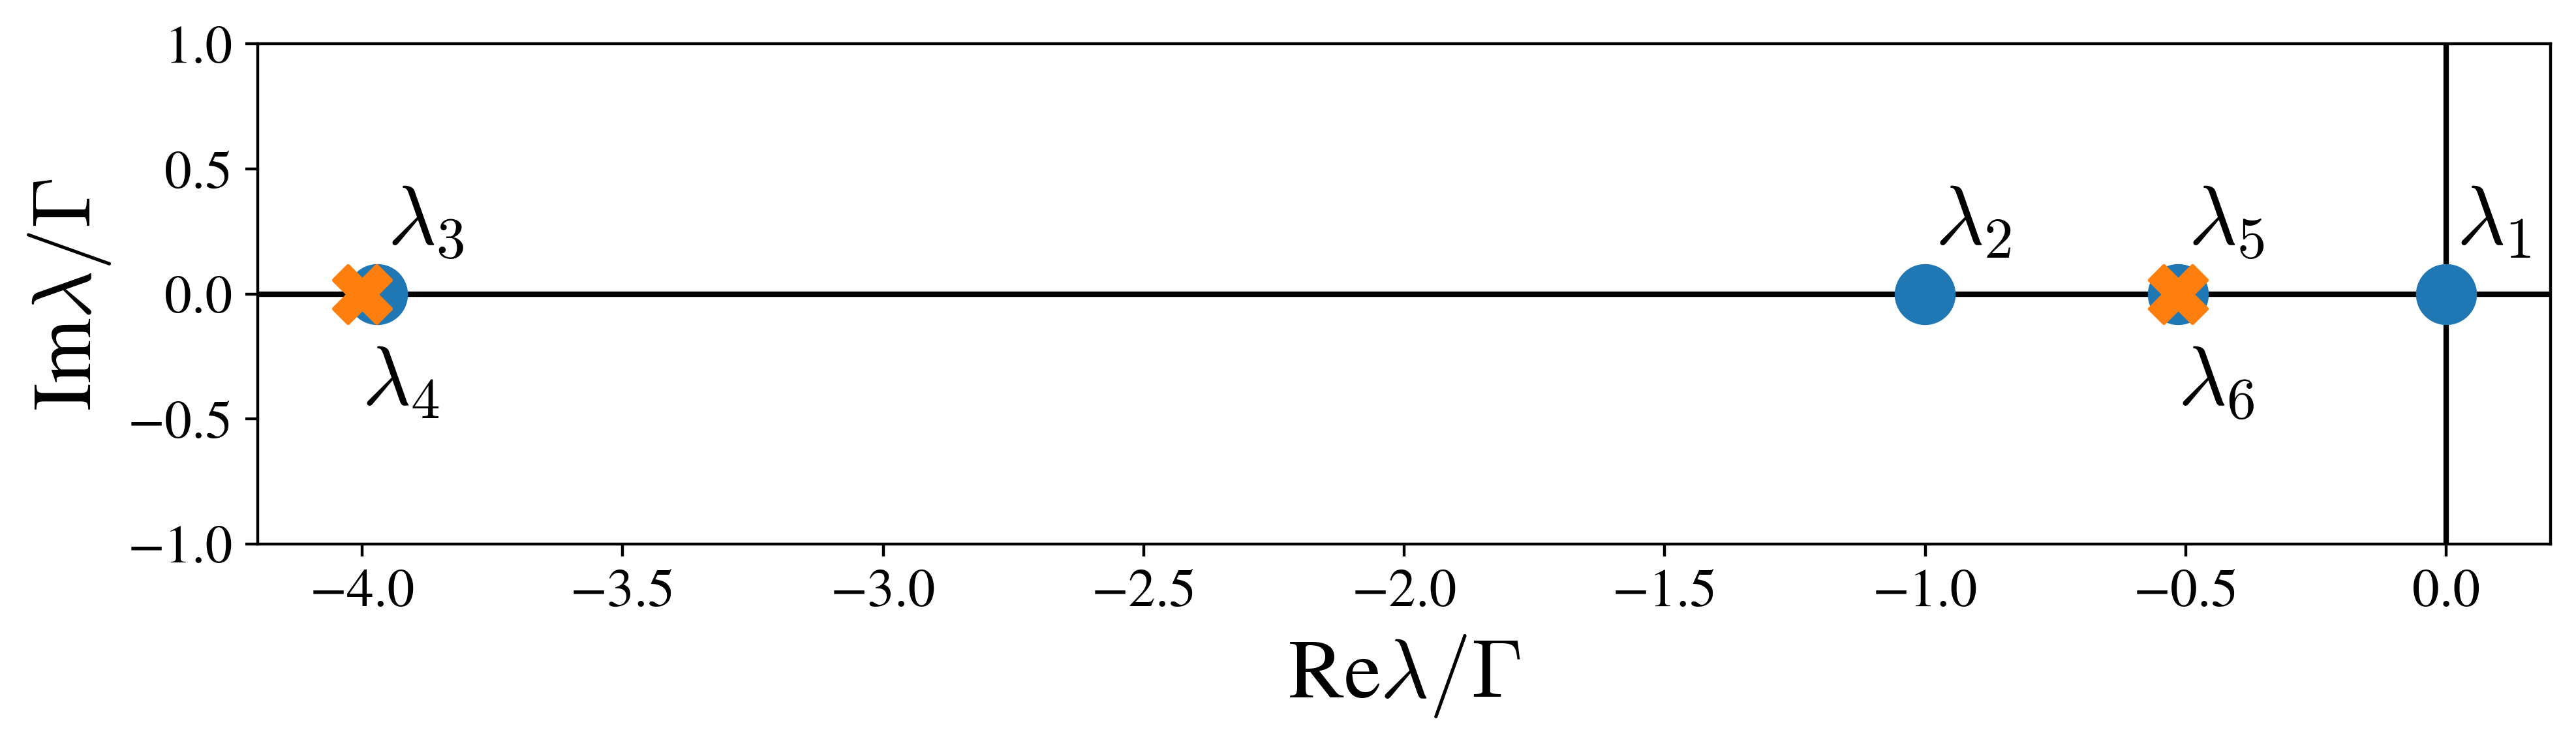
\includegraphics[width=0.8\linewidth]{figures/spectrum.png}
    \caption{The spectrum of the Liouvillian at the exceptional point.}
    \label{fig:spec}
\end{figure}

Using equation~\eqref{eq:genmodeFL}, the evolution of the system can be given in terms of the eigenvalues and generalized eigenvectors of $L$. Outside of an exceptional point, the Liouvillian is diagonalizable, and the terms are purely exponential. The evolution of the density operator is then given by
\begin{equation}\label{eq:dynnonep}
    \ket{\rho(t)}\rangle = \ket{\rho_{ss}}\rangle + \sum_{i=2}^6 e^{\lambda_i t} \langle\braket{\sigma_i|\rho(0)}\rangle \ket{\rho_i}\rangle
\end{equation}
where $\ket{\rho_{ss}}\rangle = \langle\braket{\sigma_1|\rho(0)}\rangle \ket{\rho_1}\rangle$ is the steady state of the system, due to the zero eigenvalue $\lambda_1=0$.

At the exceptional point, the Jordan form of $L$ and its exponential $e^{Jt}$ have to be evaluated. Since the EP is of order two, this results in a $2\times2$ Jordan block. This is the only EP, which means that rest of the Jordan form is diagonal. Using equations~\eqref{eq:jordan} and~\eqref{eq:expjordan}, this results in the following Jordan form and Jordan exponential:

\begin{equation}
    J = \begin{bmatrix} 0 & 0 & 0 & 0 & 0 & 0 \\
                        0 & \lambda_2 & 0 & 0 & 0 & 0 \\
                        0 & 0 & \lambda_3 & 0 & 0 & 0 \\
                        0 & 0 & 0 & \lambda_4 & 0 & 0 \\
                        0 & 0 & 0 & 0 & \bar \lambda & 1 \\
                        0 & 0 & 0 & 0 & 0 & \bar \lambda \\ \end{bmatrix}, \; 
        e^{Jt} = \begin{bmatrix} 1 & 0 & 0 & 0 & 0 & 0 \\
            0 & e^{\lambda_2t} & 0 & 0 & 0 & 0 \\
            0 & 0 & e^{\lambda_3t} & 0 & 0 & 0 \\
            0 & 0 & 0 & e^{\lambda_4t} & 0 & 0 \\
            0 & 0 & 0 & 0 & e^{\bar \lambda t} & t \\
        0 & 0 & 0 & 0 & 0 & e^{\bar \lambda t} \\ \end{bmatrix},
\end{equation}
since $\lambda_1 = 0$.

Furthermore, the Jordan chain vector $\ket{\rho'}\rangle$ defined by $(L - \bar\lambda I)\ket{\rho'}\rangle = \ket{\bar\rho}\rangle$ and its corresponding row in $M^{-1}$, $\langle\bra{\sigma'}$, need to be evaluated. Inserting these vectors into equation~\eqref{eq:genmodeFL}, the evolution of the density operator can be shown to be given by
\begin{equation}\label{eq:dynep}
    \begin{aligned}
        \ket{\rho(t)}\rangle = &\ket{\rho_{ss}}\rangle + \sum_{i=2}^4 e^{\lambda_i t} \langle\braket{\sigma_i|\rho(0)}\rangle \ket{\rho_i}\rangle \\ 
                               & + e^{\bar \lambda t}\left\{\langle\braket{\bar\sigma|\rho(0)}\rangle + t\langle\braket{\sigma'|\rho(0)}\rangle \right\}\ket{\bar \rho}\rangle \\ 
                               & + e^{\bar\lambda t} \langle\braket{\sigma'|\rho(0)}\rangle\ket{\rho'}\rangle.
    \end{aligned}
\end{equation}
By numerically calculating the generalized eigenvectors and the corresponding rows in $M^{-1}$, the dynamics at non-EP and at EP given by equations~\eqref{eq:dynnonep} and~\eqref{eq:dynep}, could be implemented. The results were then compared with a numerical ODE-solver, see figure~\ref{fig:minevsint}.

\begin{figure}[H]
    \centering
    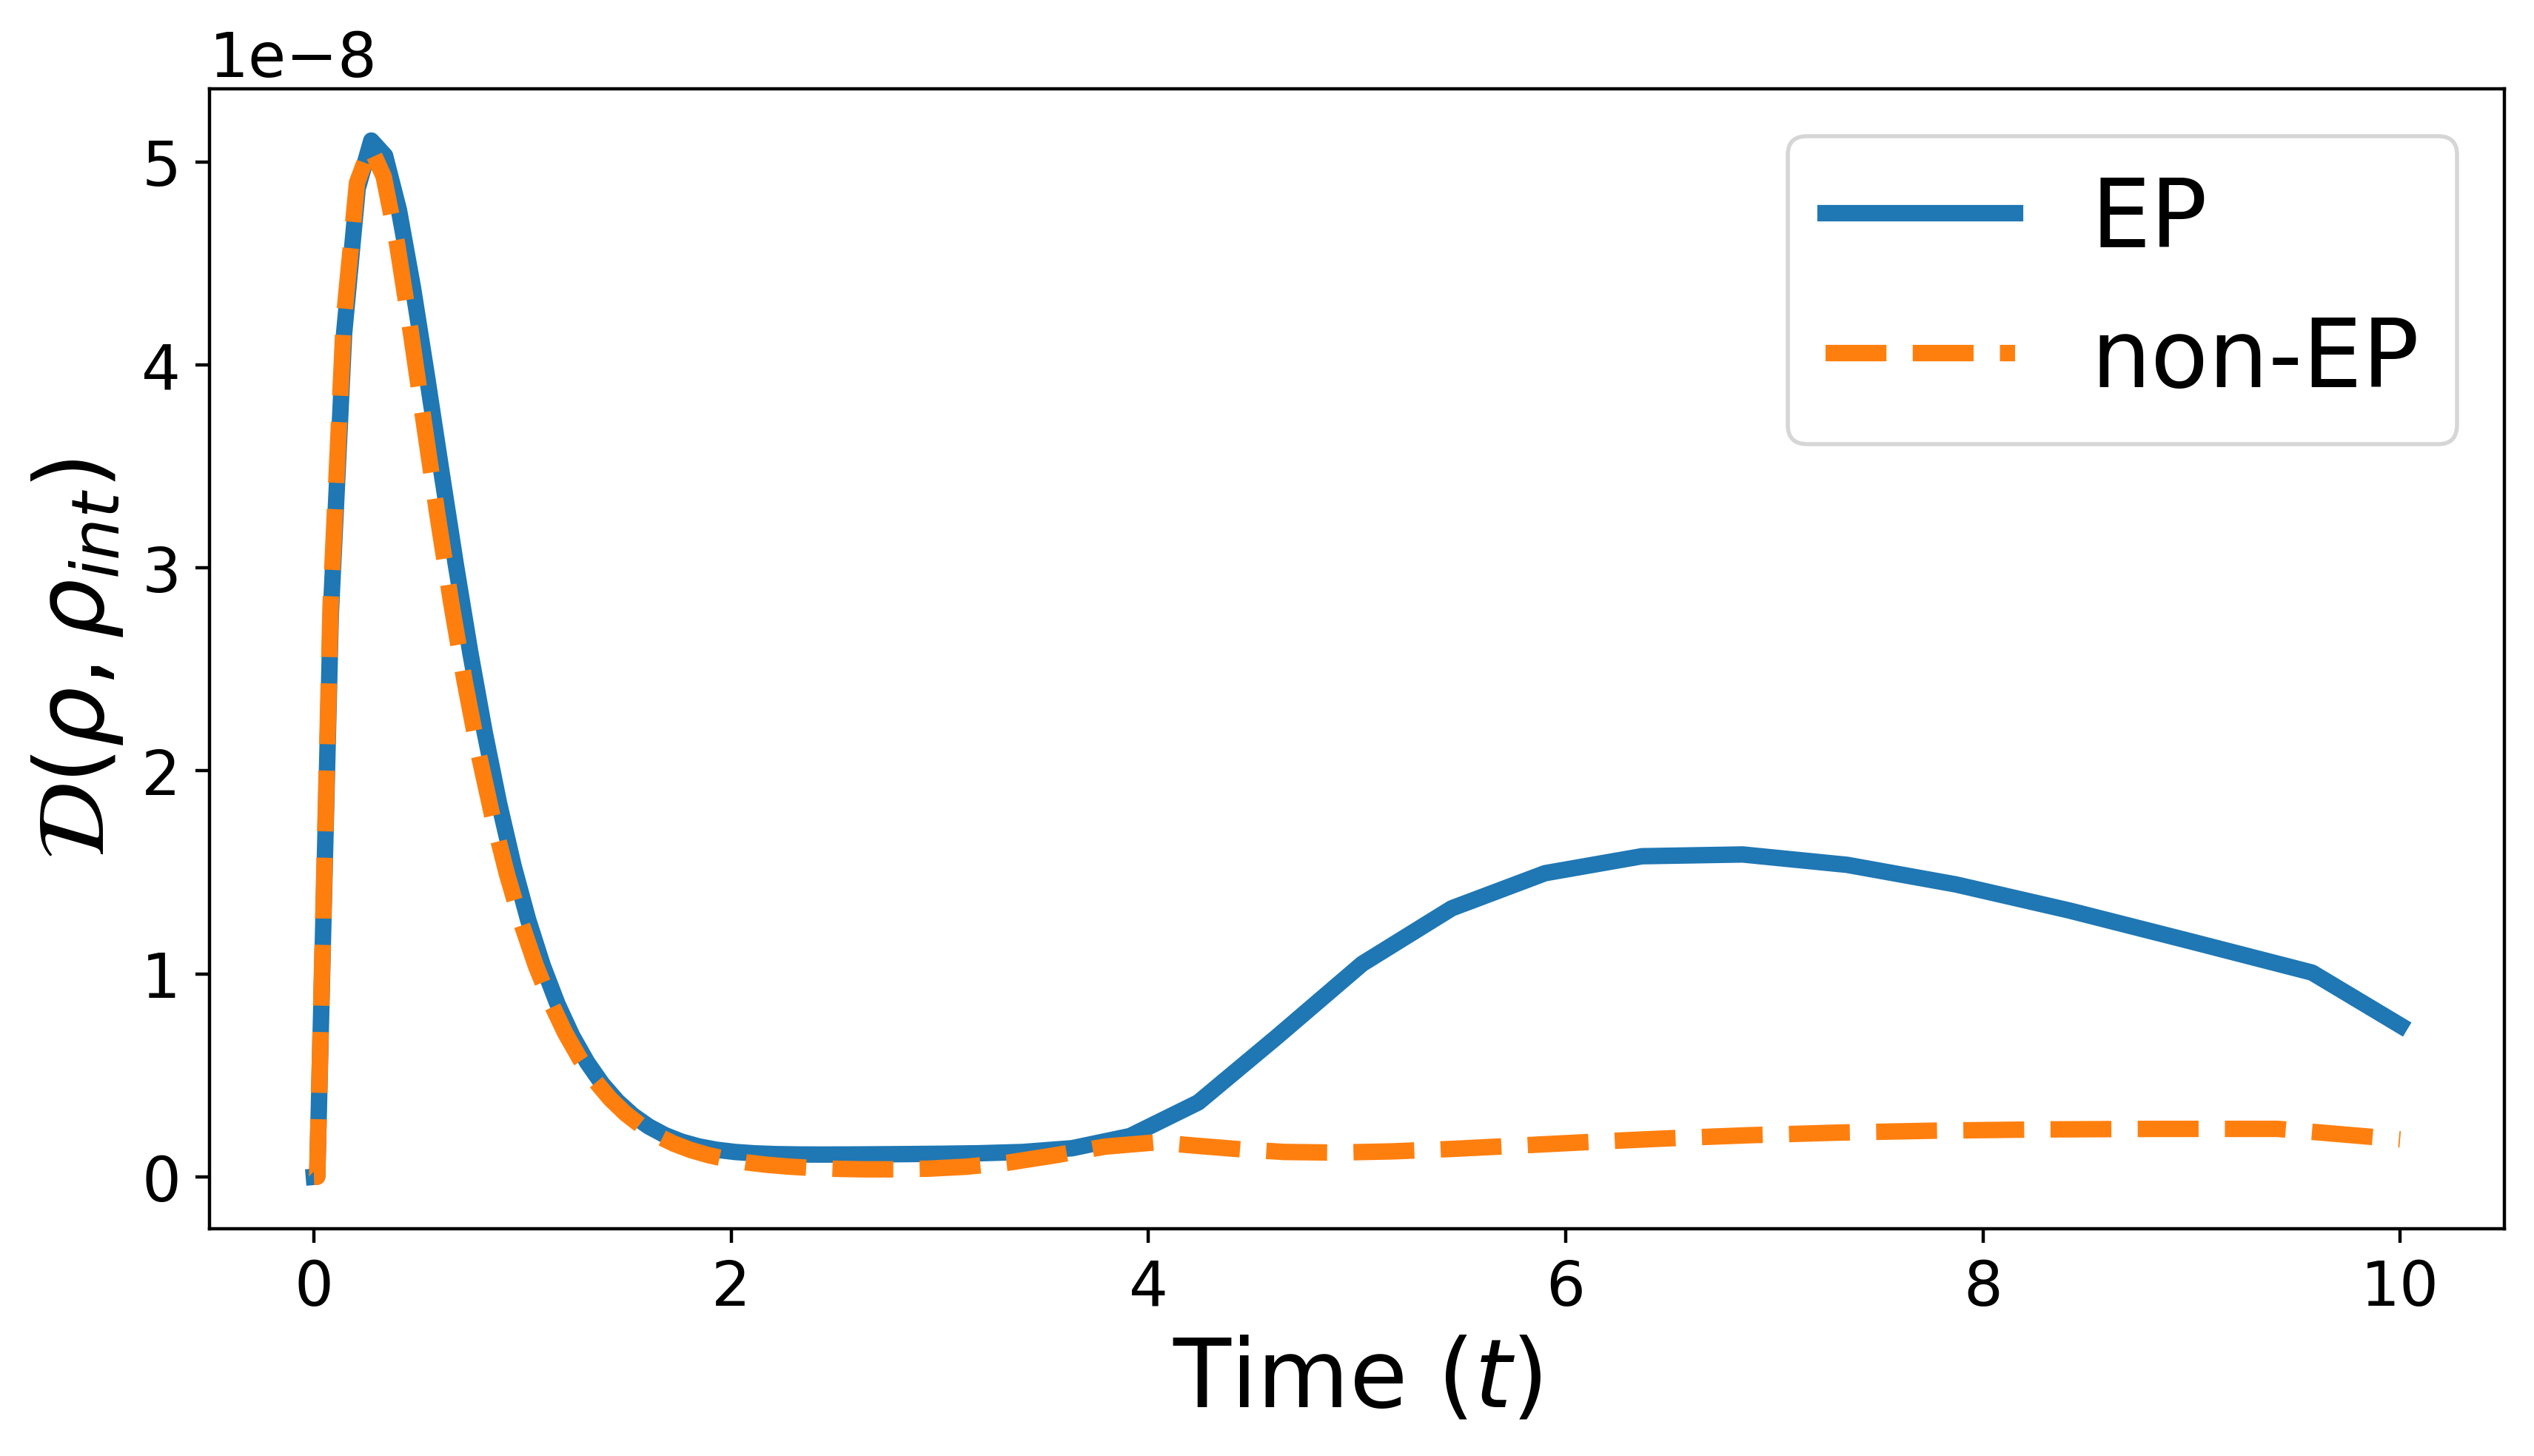
\includegraphics[width=0.7\linewidth]{figures/minevsint.png}
    \caption{The relative distance $\mathcal{D}(\ket{\rho}\rangle, \ket{\rho_\text{int}}\rangle) = \frac{||\ket{\rho}\rangle - \ket{\rho_\text{int}}\rangle||_1}{||\ket{\rho_\text{int}}\rangle||_1}$ between the density matrices calculated with the implemented methods and with a numerical solver. The two lines represent the distances at the EP and away from the EP, using the corresponding implemented methods for each case. The numerical solver was set to an absolute and relative tolerance of $10^{-10}$ and $10^{-6}$ respectively.}
    \label{fig:minevsint}
\end{figure}


With a clear picture of the analytical dynamics and numerically calculated eigenvalues and generalized eigenvectors at hand, simulations of the current in the parallel dot system could be done. As discussed in the theory section, any relevant observable of the system can be obtained from the density operator. For the parallel dot system, the main observable is the current $\hat I$, which is described in terms of the jump operator. Using equation~\eqref{eq:expec}, the current can be calculated with $\braket{\hat I(t)} = \tr{(\hat \rho(t)\hat I)}$. Implementing this numerically, the current through the quantum dot system for varying parameters and initial conditions could be simulated. The first simulation involved sitting at an EP and choosing initial conditions in terms of the generalized eigenvectors, see figure~\ref{fig:diffrho0}. In figure~\ref{fig:diffde}, the dynamics of the current at and slightly away from the exceptional point was simulated.
\begin{figure}[H]
    \centering
    \begin{minipage}[t]{0.48\textwidth}
        \centering
        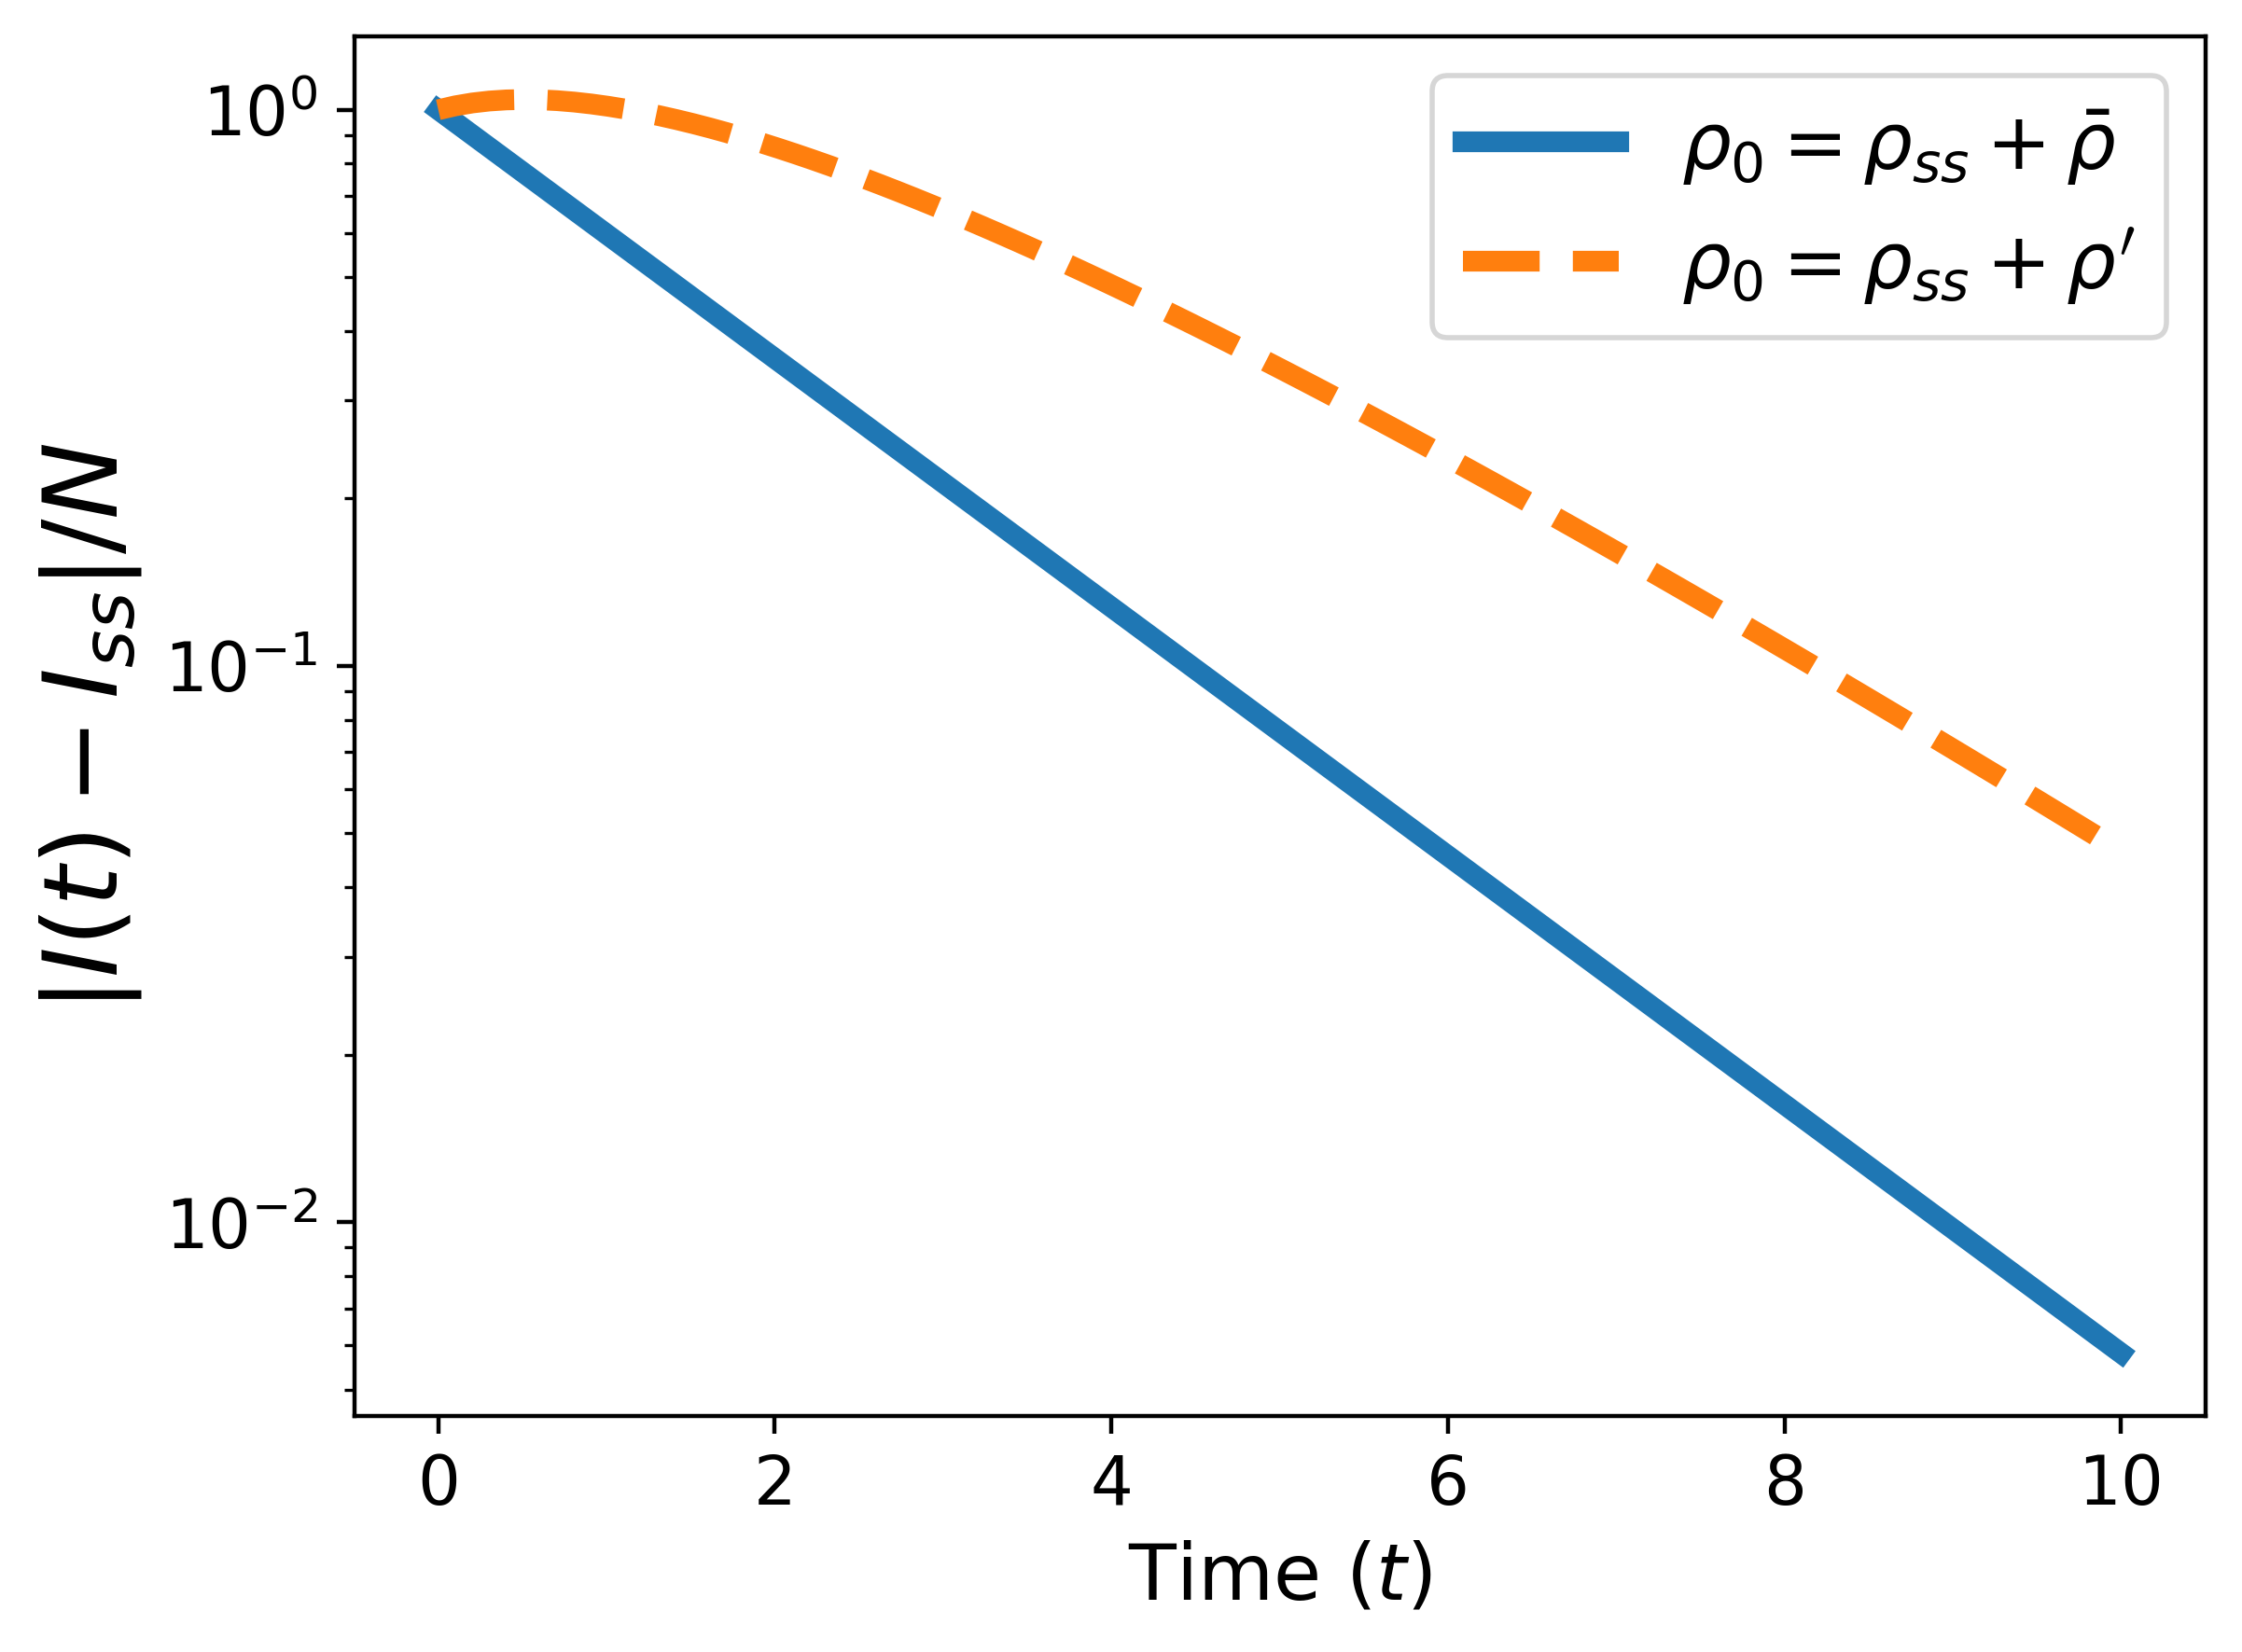
\includegraphics[width=\textwidth]{figures/current_diff_rho_0.png}
        \caption{The decay of the current towards the steady state current $I_{ss}$ in a log plot. The simulations were done at the EP with different initial conditions. A normalization by $N=|I(0) - I_{ss}|$ was done such that each curve is unity for $t=0$.}
    \label{fig:diffrho0}
    \end{minipage}\hfill
    \begin{minipage}[t]{0.48\textwidth}
        \centering
        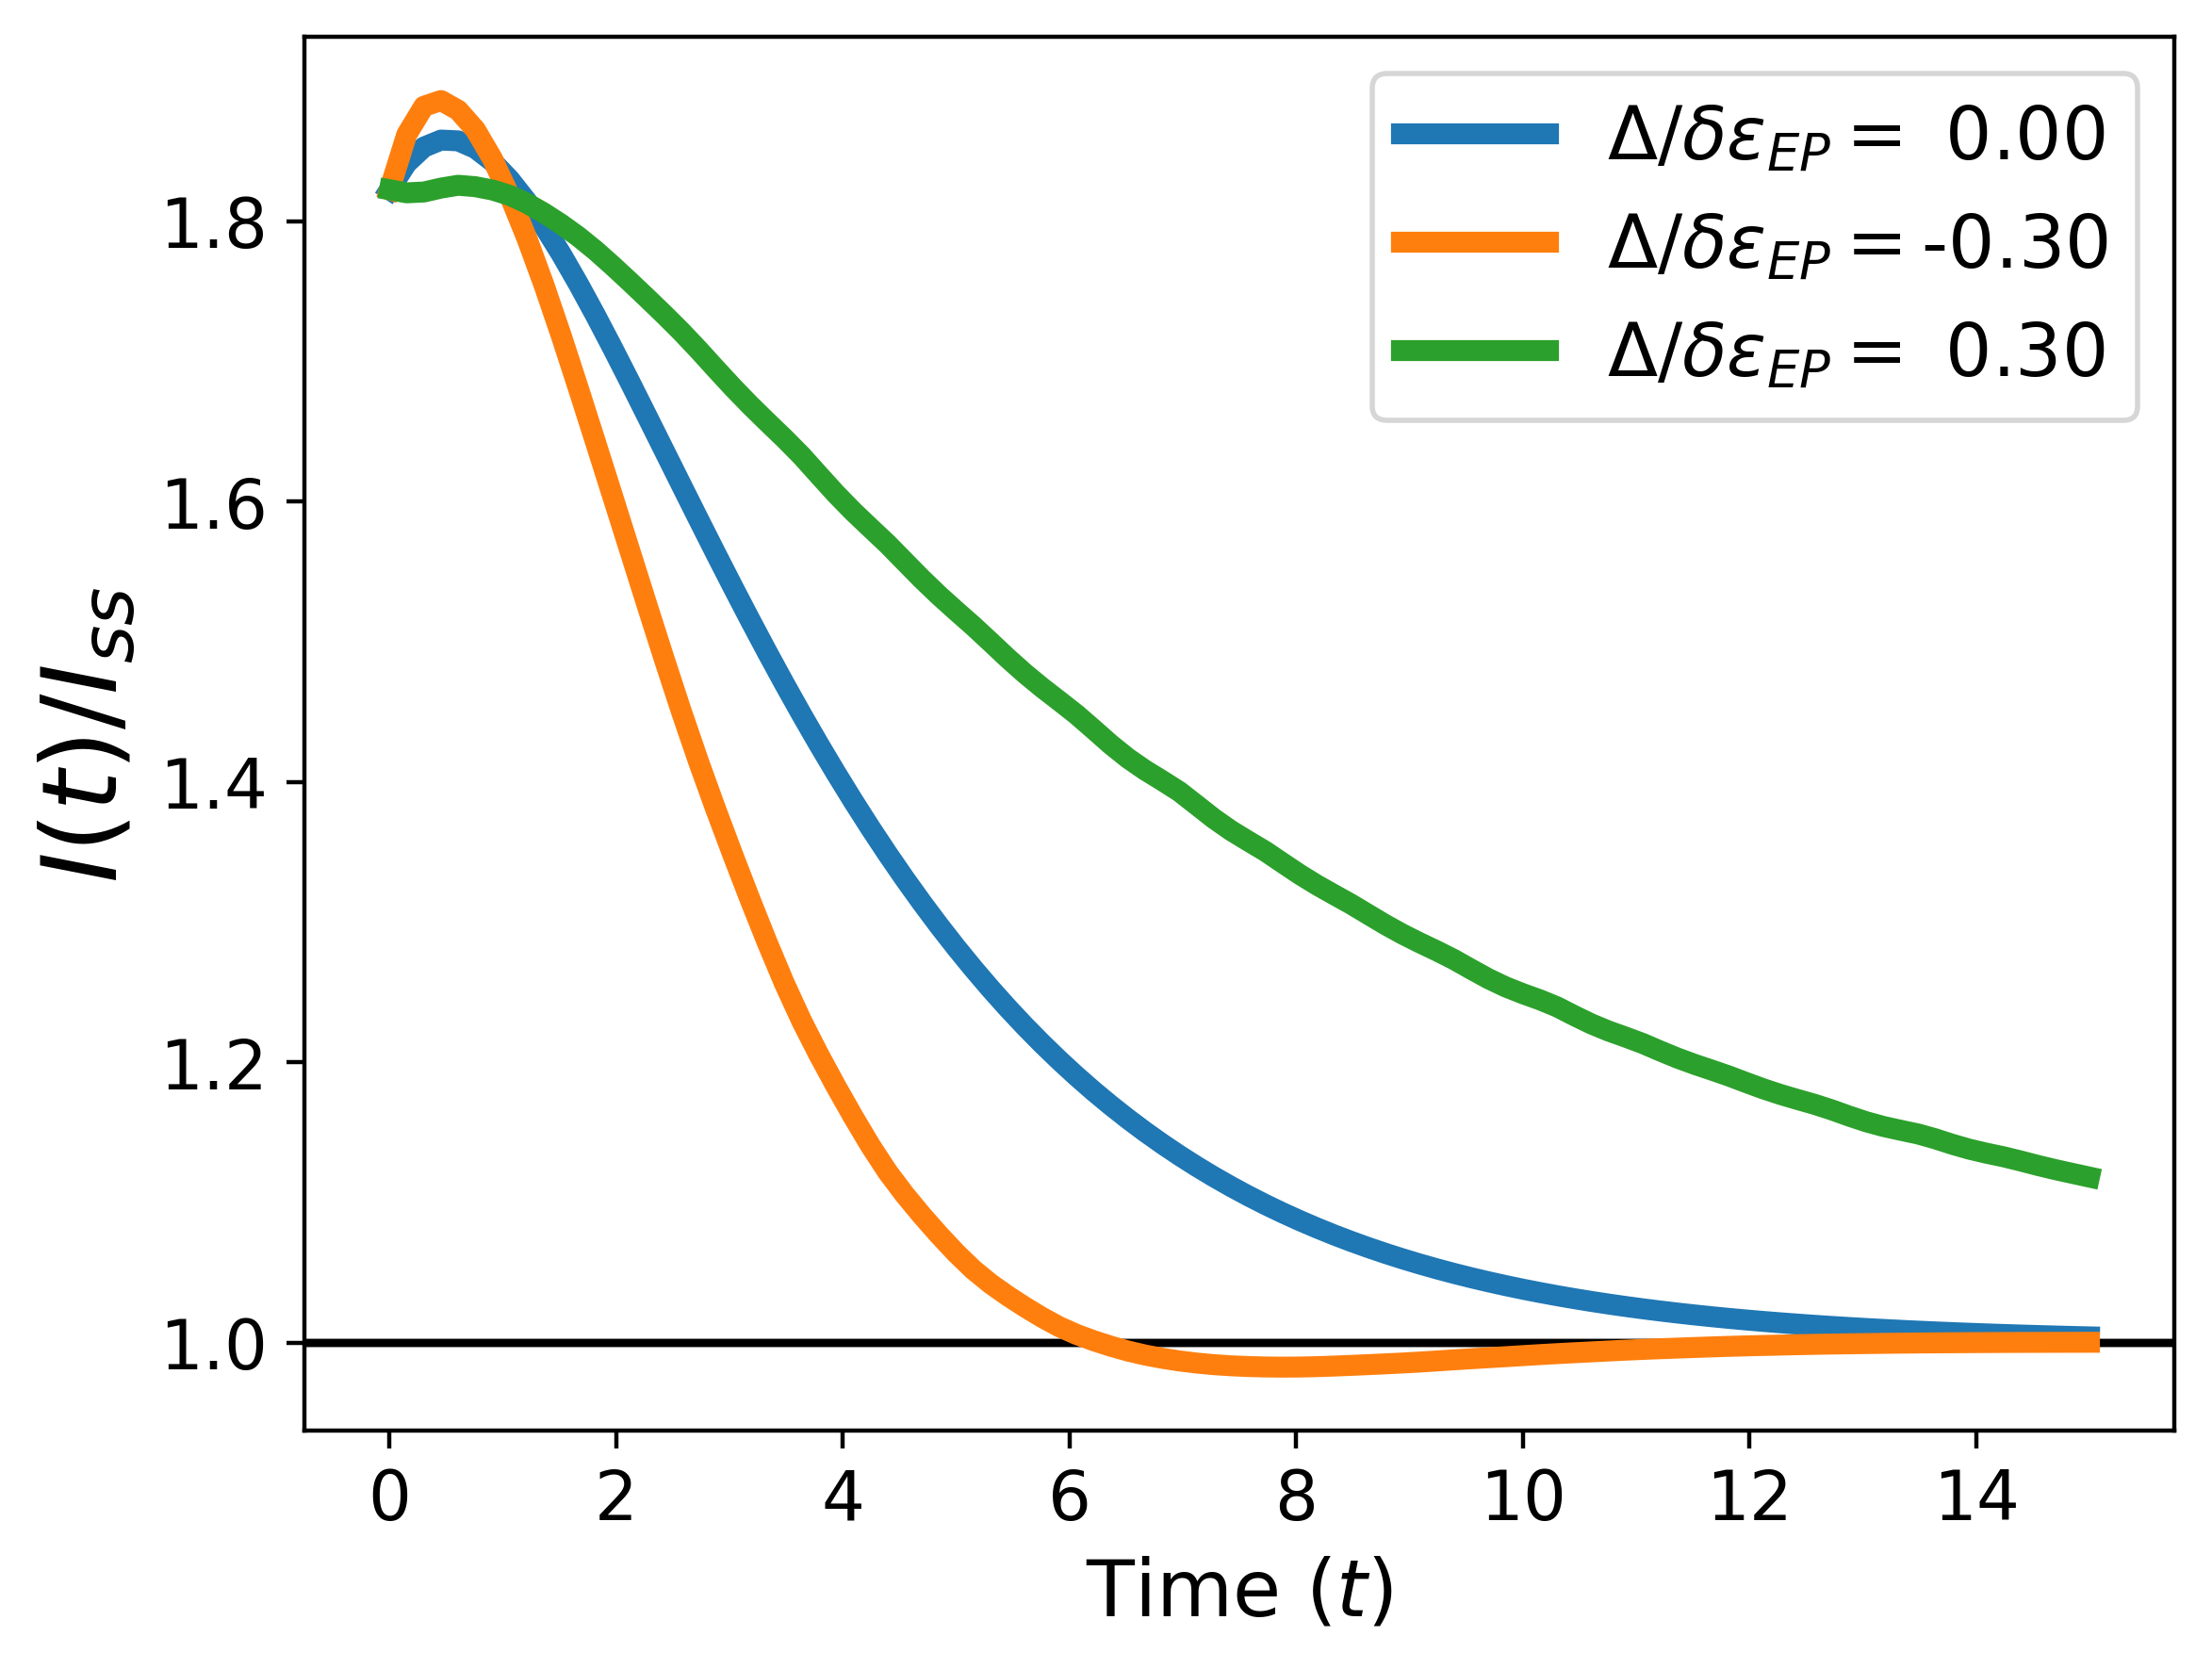
\includegraphics[width=\textwidth]{figures/curr_diff_de.png}
        \caption{The current over time for different $\delta\epsilon$, normalized by the steady state current $I_{ss}$. The solid, blue curve correspond to the system being at the EP, while the other two are slightly away from it. All simulations were done with the same initial condition.}
    \label{fig:diffde}
    \end{minipage}\hfill
\end{figure}



\end{document}
